
\documentclass[12pt]{article}              
\usepackage[margin=2.0cm]{geometry}
\usepackage{setspace,relsize}               
\usepackage{moreverb}                        
\usepackage{url}
\usepackage{hyperref}
\hypersetup{colorlinks=true,citecolor=blue}
\usepackage{amsmath}
\usepackage{mathtools} 
\usepackage{amssymb}
\usepackage{indentfirst}
\usepackage[authoryear,round]{natbib}
\bibliographystyle{apalike}
\usepackage[pdftex]{lscape}
\usepackage[toc,page]{appendix}
% \usepackage{float}
% \usepackage{longtable}
% \usetikzlibrary{arrows}
%%%%
\title{
Stochastic Multistrain Dengue model
}           
\author{
Flavio Code\c{c}o Coelho \\
\\
\& \\
Luiz Max de Carvalho \\
}

\date{}
% Notation defs
\def \rr {$R_{t}\ $}


\begin{document}                                  


%
\maketitle


\section*{Multi-strain dynamics}

In this paper we propose a stochastic 4-serotype SIR model with 
cross-immunity to describe multi-strain Dengue dynamics. 
The model permits up to 4 dengue infections 
with reduced susceptibility after the first Dengue episode due to cross 
immunity. 
Immunity to each serotype is considered complete and permanent. 
Figure \ref{fig:sde_blocks} depicts all 48 possible states and 64 
state-transitions included in the model.

          \begin{figure}
 \centering
 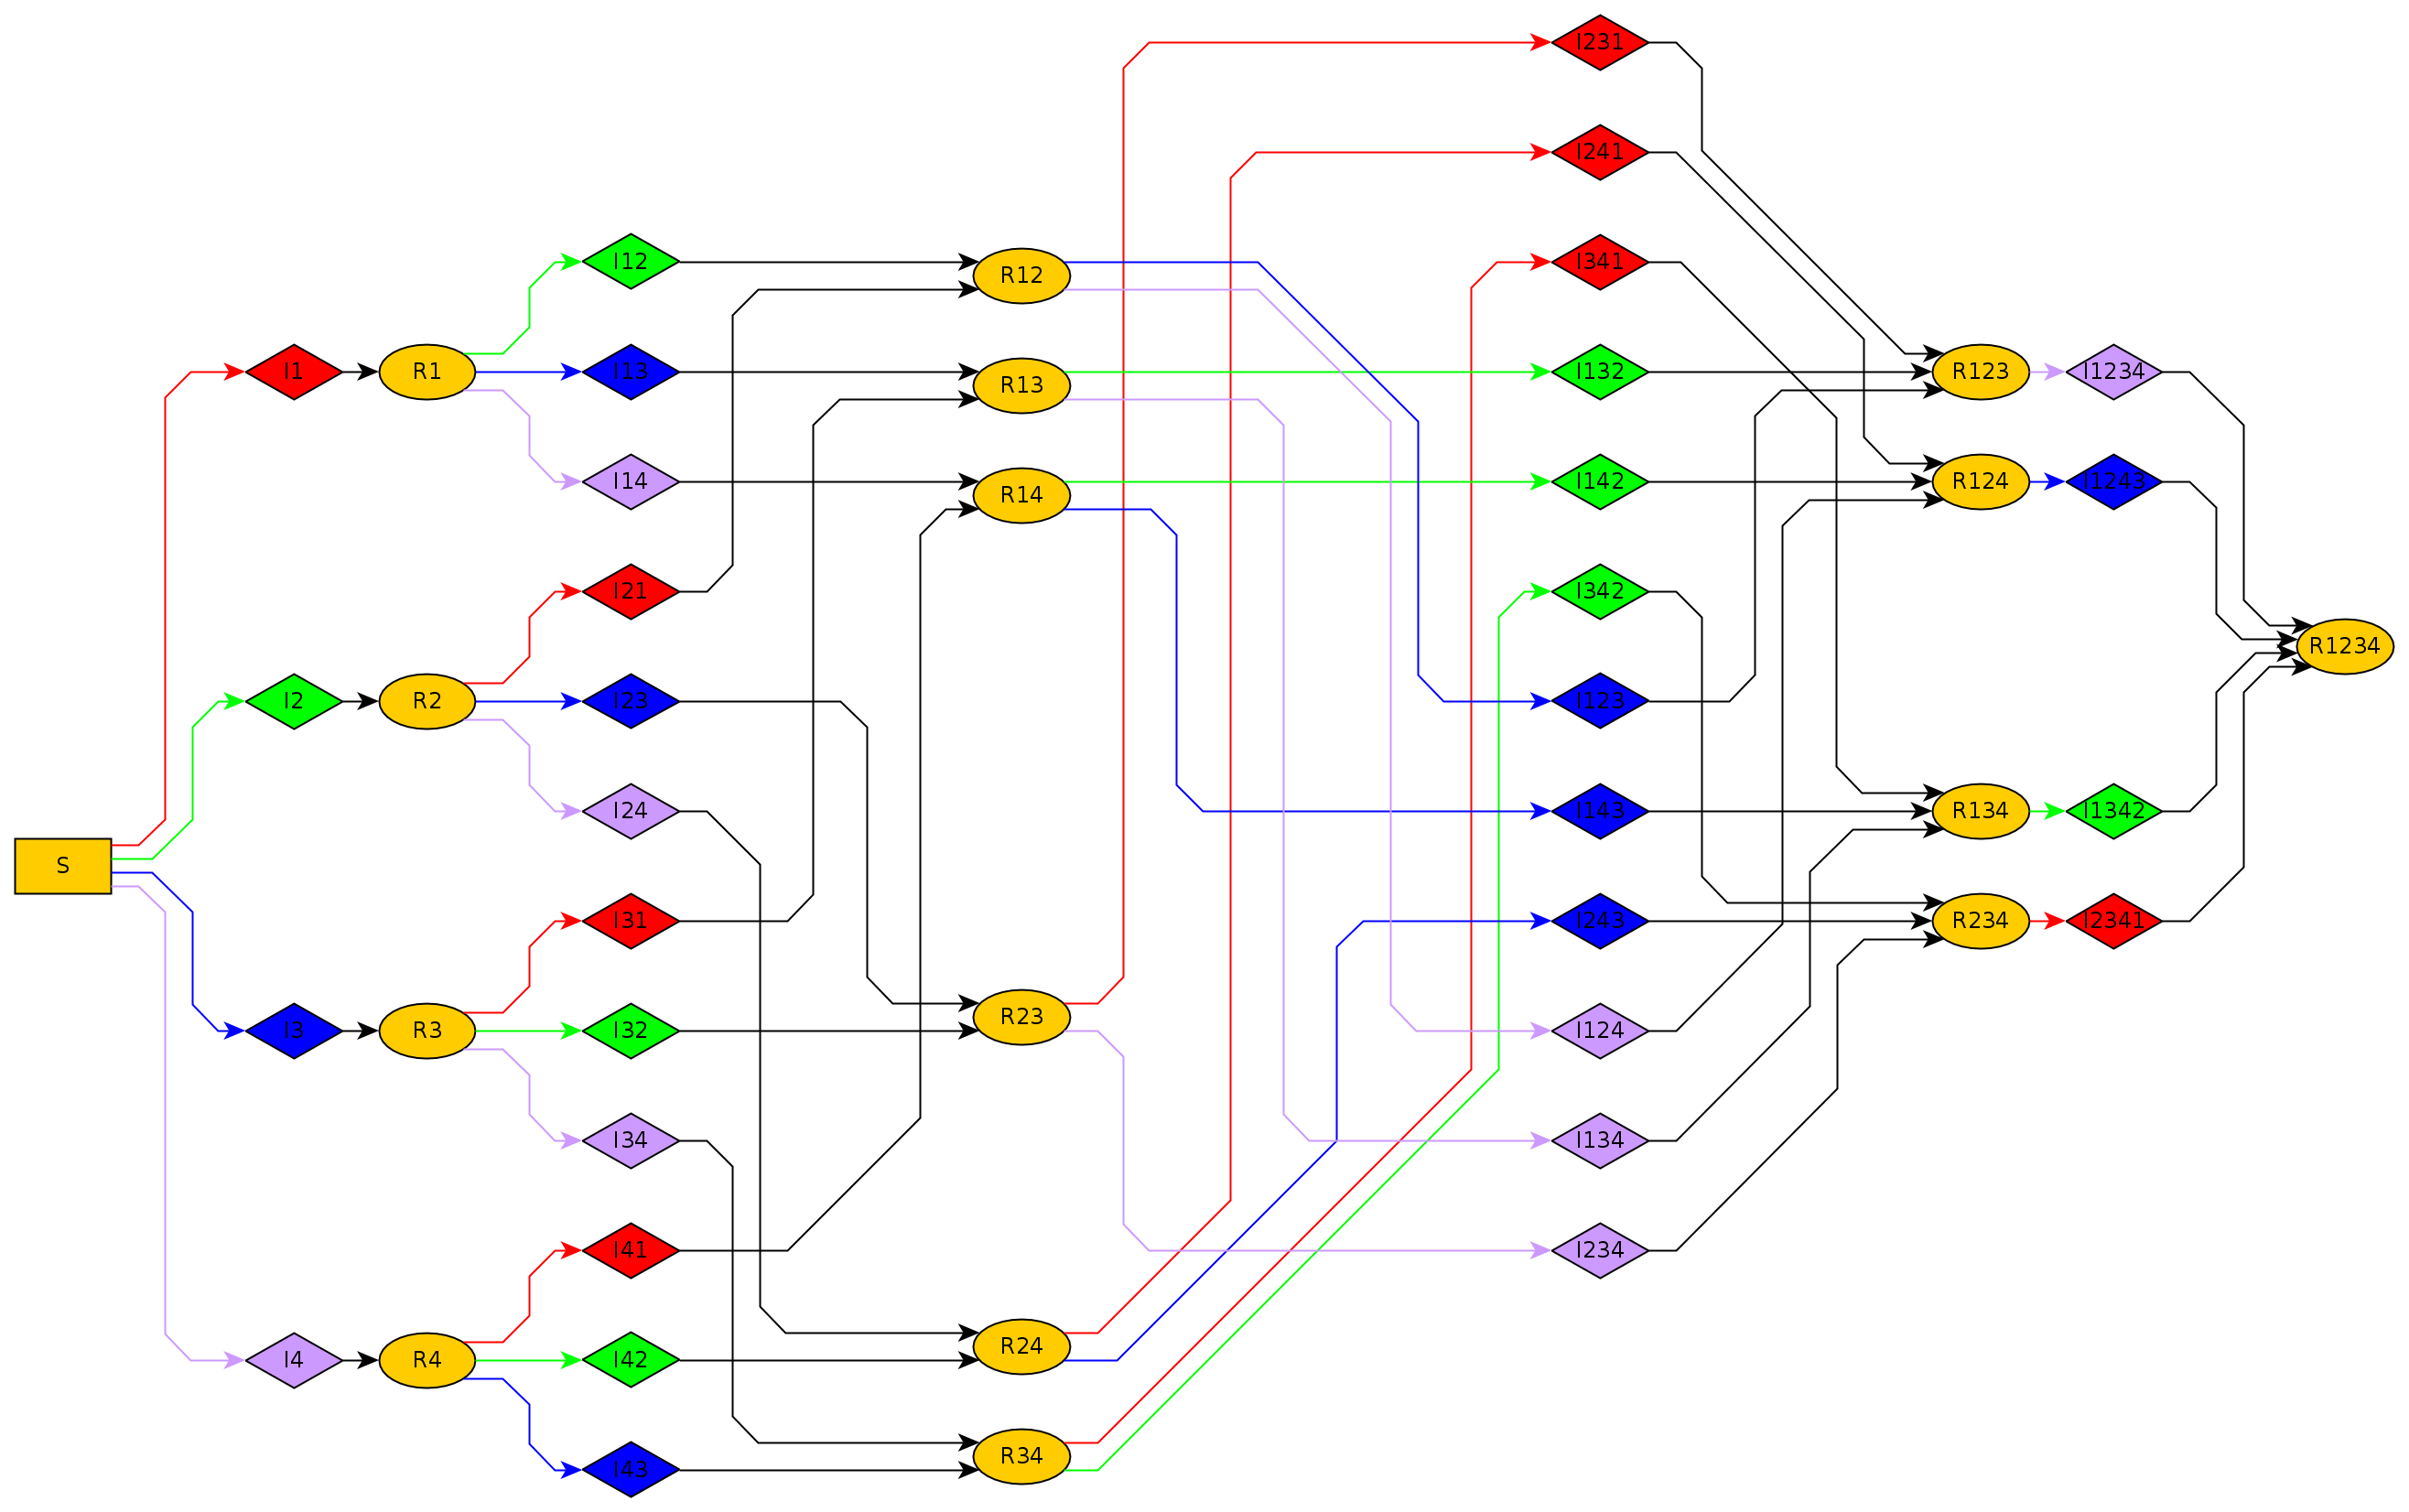
\includegraphics[width=16cm]{Dengue4.png}

 \caption{Block diagram detailing the stochastic model. Infected individuals 
with different Dengue viruses are represented by different colors. Infections 
are also represented by colored arrows matching the virus type.}
 \label{fig:sde_blocks}
\end{figure}


Let $S$ be individuals susceptible to all 4 types of dengue, $I_i$ infectious 
with Dengue type $i$ and $R_i$ individuals recovered from Dengue type $i$. 
Infectious individuals already on their secondary and later Dengue infections 
are represented by multiple indices. For example, $I_{[23]1}$ is an individual 
which has had Dengues type 2 and 3 in the past -- and therefore is immune to 
them -- and is currently transmitting Dengue 1. 
The index outside the bracket 
denotes current infection. Recovered individuals indices denote their immunity, 
so for instance $R_{123}$ is an individual which is immune to Dengue types 1, 2 
and 3, but not to 4. Let $I_{*i} = \sum I_{[\ldots]i}$ with $[\ldots]$ 
representing exposure history of the infected individual which can vary from 0 
to 3 in length. 
All individuals are born to the $S$ state and birth and death 
rates are equal.

The possible state-transitions and their  propensities are listed in table 
\ref{tab:trans}.
\begin{table}
\caption{
\bf{State-transitions and probabilities: $P(\Delta X(t)|X(t))$}. The 
transitions are summarized below. Fully expanded, the system contemplates 64 
possible state transitions, as can be verified in figure \ref{fig:sde_blocks}. 
$^\dag$: $P(\cdot)$ is the sum of the probabilities of all possible state 
changing transitions.
}
\label{tab:trans}
\begin{center}
\begin{tabular}[c]{l|l|l|l}
\hline
Transition & Probability & State Change & Description\\
\hline
$S \rightarrow I_i$ & $\beta S I_{*i} \Delta t$ & $\Delta S(t)=-1,\, \Delta 
I_i(t) = 1$ 
& Primary infection \\
$I_i \rightarrow R_i$ & $\sigma I_i \Delta t$ & $\Delta I_i(t)=-1,\, \Delta 
R_i(t) = 1$ 
& Primary recovery\\
$R_i \rightarrow I_{[i]j}$ & $\beta \delta R_i I_{*j}\Delta t$ & $\Delta 
R_i(t)=-1,\, 
\Delta I_{[i]j}(t) = 1$ & Secondary infection\\
$I_{[i]j} \rightarrow R_{ij}$ & $\sigma I_{[i]j}\Delta t$ &$\Delta 
I_{[i]j}(t)=-1,\, 
\Delta R_{ij}(t) = 1$& Secondary recovery\\
$R_{ij} \rightarrow I_{[ij]k}$ & $\beta \delta R_{ij} I_{*k}\Delta t$ &$\Delta 
R_{ij}(t)=-1,\, \Delta I_{[ij]k}(t) = 1$& Tertiary infection\\
$I_{[ij]k} \rightarrow R_{ijk}$ & $\sigma I_{[ij]k}\Delta t$ &$\Delta 
I_{[ij]k}(t)=-1,\, \Delta R_{ijk}(t) = 1$& Tertiary recovery\\
$R_{ijk} \rightarrow I_{[ijk]l}$ & $\beta \delta R_{ijk} I_{*l}\Delta t$ 
&$\Delta 
R_{ijk}(t)=-1,\, \Delta I_{[ijk]l}(t) = 1$& Quaternary infection\\
$I_{[ijk]l} \rightarrow R_{ijkl}$ & $\sigma I_{[ijk]l}\Delta t$ & $\Delta 
I_{[ijk]l}(t)=-1,\, \Delta R_{ijkl}(t) = 1$ & Quaternary recovery\\
$\rightarrow S$ & $\mu N\Delta t$ & $\Delta S = 1$ & Birth\\
$All \rightarrow$ & $\mu N\Delta t$ & $\Delta S = \Delta I_* = \Delta R_* = -1$ 
& Death\\
No transition & $1-P(\cdot)^\dag$ & No change & ---\\
\hline
\end{tabular}
\end{center}

\end{table}

The model is implemented as a continuous time Markov jump process. Let
$$\overrightarrow{X}(t) = [S(t), I_1(t), I_2(t), \ldots, R_{1234}(t)]$$ 
be the 
state of the system at the time $t$. $\sum X(t) = N, \forall t$ with $N$ being 
the population size. 
The system is written as a forward Kolmogorov differential equation, which in 
matrix form looks like
\begin{equation}
\frac{dP_X(t)}{dt} = Q P_X(t) 
\end{equation}

Where $P_X(t)$ is  the matrix of transition probabilities (given in table 
\ref{tab:trans}) and Q is the generator matrix, whose non-zero values are also 
given in table \ref{tab:trans} (in the state change column). The full formula 
and matrices are ommited due to their large sizes.

\subsection*{Expected Change and Covariance Matrix}

It is useful to calculate the expected change and the covariance matrix for the 
changes $\Delta X = [\Delta S, \Delta I_1, \Delta I_2, \Delta I_3, \Delta I_4,$
$\Delta R_1, \Delta R_2, \Delta R_3, \Delta R_4,\Delta I_{12}, \Delta I_{13},
\Delta I_{12}, \Delta I_{13}, 
\Delta I_{14}, \Delta I_{21}, \Delta I_{23}, \Delta I_{24}, \Delta I_{31},$
$\Delta I_{32}, 
\Delta I_{34}, \Delta I_{41}, \Delta I_{42}, \Delta I_{43}, \Delta R_{12}, 
\Delta R_{13}, \Delta R_{14}, \Delta R_{23}, \Delta R_{24}, \Delta R_{34},
\Delta I_{231}, \Delta I_{241}, \Delta I_{341}, \Delta I_{132}, \Delta I_{142},$
$\Delta I_{342}, \Delta I_{123}, \Delta I_{143}, \Delta I_{243}, \Delta I_{124},
\Delta I_{134}, \Delta I_{234}, \Delta R_{123}, \Delta R_{124}, \Delta R_{134},
\Delta R_{234}, \Delta I_{1234}, \Delta I_{1243}, \Delta I_{1342},$\\
$\Delta I_{2341},\Delta R_{1234}]^T$.


Thus from the probabilities of table \ref{tab:trans},

\begin{equation}
 E(\Delta X)=\sum_X p_i \Delta X_i=
\begin{pmatrix}
-\beta S I_{*1} + \mu N -\mu S\\
\vdots\\
\beta S I_{*4} + \mu N -\mu S\\
\beta S I_{*1} -\sigma I_1 -\mu I_1\\
\vdots\\
\beta S I_{*4} -\sigma I_4 -\mu I_4\\
\sigma I_1 - \beta \delta R_1 I_{*j} -\mu R_1\\
\vdots\\
\sigma I_4 - \beta \delta R_4 I_{*j} -\mu R_4\\
\beta \delta R_i I_{[i]j} - \sigma I_{[i]j} -\mu I_{[i]j}\\ 
\sigma I_{[i]j} - \beta \delta R_{ij} I_{*k} - \mu R_{ij}\\
\beta \delta R_{ij} I_{*k} -\sigma I_{[ij]k} -\mu I_{[ij]k}\\ 
 \end{pmatrix}
 \Delta t
\end{equation}

The expected change, $E(\Delta X)$, is a $48\times 1$ vector.
%\bibliography{lm1}
\end{document}
